This chapter describes how to simulate from our multiGLMM, and describes
a real-based dataset used as an application example. The simulation
procedure addressed in \autoref{cap:simu} is not straightforward, since
we need to simulate the outputs (failure or censor) and the
failure/censoring times, controlling for a pre-specified censorship
level. In \autoref{cap:data} a simulated dataset based on the Nordic
Cancer Union (NCU) twins data is presented as an application example.

\section{SIMULATING FROM A \(\text{multiGLMM}\)}
\label{cap:simu}

Being able to simulate some data from a model is a key task, fundamental
to assess the finite-sample properties and the estimation procedure of a
given statistical model.

The core of the simulation procedure for our multiGLMM,
\autoref{eq:model}, was proposed by \citeonline{SCHEIKE} and is
basically a four-step procedure.

In the first step, based on the set model parameters and sampled latent
effects, we compute the cause-specific failure times. The second step
(the only when that differs from the simulation procedure proposed by
\citeonline{SCHEIKE}) consists of the computation of all competing risk
probabilities as defined in \autoref{eq:model}, with the censorship
probability being computed as the complementary to guarantee that the
probabilities sum up 1 to each individual. Based on that probabilities,
we sample the outputs, i.e. the subject fails or censors, from a
multinomial probability distribution. The last and fourth step is a
somehow output overwriting to have better control of the proportion of
censorship. In this last step which individuals should be censor are
chosen by a Bernoulli process, with a fixed probability, and its
censoring times are sampled from a given Uniform probability
distribution. Algorithm~\ref{alg:algo} describes step-by-step all that
process for an arbitrary number of competing causes of failure.

\begin{algorithm}[H]
  \caption{SIMULATING FROM THE \(\text{multiGLMM}\)}
  \label{alg:algo}
\begin{algorithmic}[1]
    \State
    Set \(J\), the number of clusters/families
    \State
    Set \(n_{j}\), the number of individuals in each family
    \Comment{can be of different sizes}
    \State
    Set values to the model parameters \(\bm{\theta} =
    [\bm{\beta}~\bm{\gamma}~\bm{w}~\bm{\sigma^{2}}~\bm{\varrho}]^{\top}\)
    \State
    Sample \(J\) vectors of latent effects from
    \(\mathcal{N}_{(K-1)\times(K-1)}(\bm{0}, ~\Sigma(\bm{\sigma^{2}},
    \bm{\varrho}))\)
    \State
    Set \(\delta\)
    \Comment{cannot exceed the maximum follow-up time}
    \State
    Sample \(\varsigma\sim\text{U}(0,~1)\)
    \State
    Compute the cause-specific failure times by solving
    \[
      \varsigma = \Phi[w_{k} g(t_{k}) - X^{\top}\gamma_{k} - \eta_{k}]
      \quad\text{for } t_{k}, \quad k = 1,~2,~\dots,~K - 1
    \]
    \State
    Compute the competing risk probabilities
    \begin{align*}
      p_{kijt}
      &= \frac{\exp\{\bm{x}_{kij}\bm{\beta}_{ki} + u_{kj}\}}{
        1 +
        \sum_{m=1}^{K-1}\exp\{\bm{x}_{mij}\bm{\beta}_{mi} + u_{mj}\}}\\
      &\times
        w_{k}\frac{\delta}{2\delta t - 2t^{2}}~
        \phi\left(
        w_{k}
        \text{arctanh}\left(\frac{t-\delta/2}{\delta/2}\right)
        - \bm{x}_{kij}\bm{\gamma}_{ki} - \eta_{kj}
        \right),\\
      p_{Kijt}
      &= 1 - \sum_{k = 1}^{K - 1} p_{kijt}, \quad k = 1,~2,~\dots,~K -1
    \end{align*}
    \State
    Sample \(J\times n_{j}\) vectors from a
    \(\text{Multinomial}(p_{1ijt},~p_{2ijt},~\dots,~p_{Kijt})\)
    \State
    If \(t_{kij} = \delta\), subject moves to class K
    \Comment{any failure at time \(\delta\) is censored}
    \State
    Set a censoring probability, \(cp\)
    \Comment{larger than actual proportion of censored}
    \State
    Sample which individuals will be censored from a
    \(\text{Bernoulli}(cp)\)
    \State
    For the censored individuals, sample the censoring times from a
    \(\text{U}(0,~\delta + 30)\)
    \State
    \Return
    To each individual, its failure/censoring time and from which
    cause-specific it is
  \end{algorithmic}
\end{algorithm}
\vspace{-.75cm}
\begin{footnotesize}
  \begin{center}
    SOURCE: The author (2020).
  \end{center}
\end{footnotesize}

\begin{figure}[H]
  % \vspace{0.35cm}
  \setlength{\abovecaptionskip}{.0001pt}
  \caption{FAILURE (\(y_{1},~y_{2}\)) AND CENSORING (\(y_{3}\)) TIMES
    FOR 200 PAIRS OF TWINS SAMPLED FROM A MODEL \dots}
  \vspace{0.425cm} \centering
  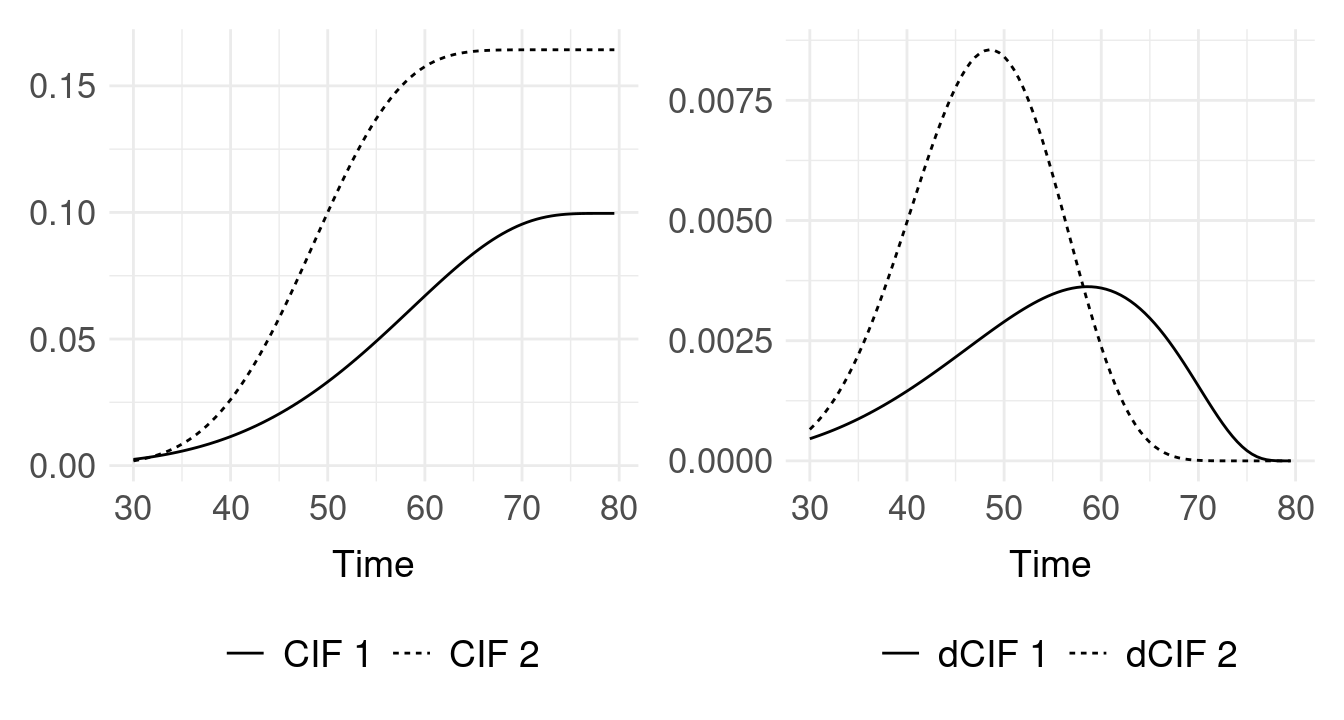
\includegraphics[width=\textwidth]{datasimucif-1.png}
  \\
  \vspace{0.45cm}
  \begin{footnotesize}
    SOURCE: The author (2020).
  \end{footnotesize}
  \label{fig:datasimucif}
\end{figure}

\begin{figure}[H]
  % \vspace{0.35cm}
  \setlength{\abovecaptionskip}{.0001pt}
  \caption{FAILURE (\(y_{1},~y_{2}\)) AND CENSORING (\(y_{3}\)) TIMES
    FOR 200 PAIRS OF TWINS SAMPLED FROM A MODEL \dots}
  \vspace{0.425cm} \centering
  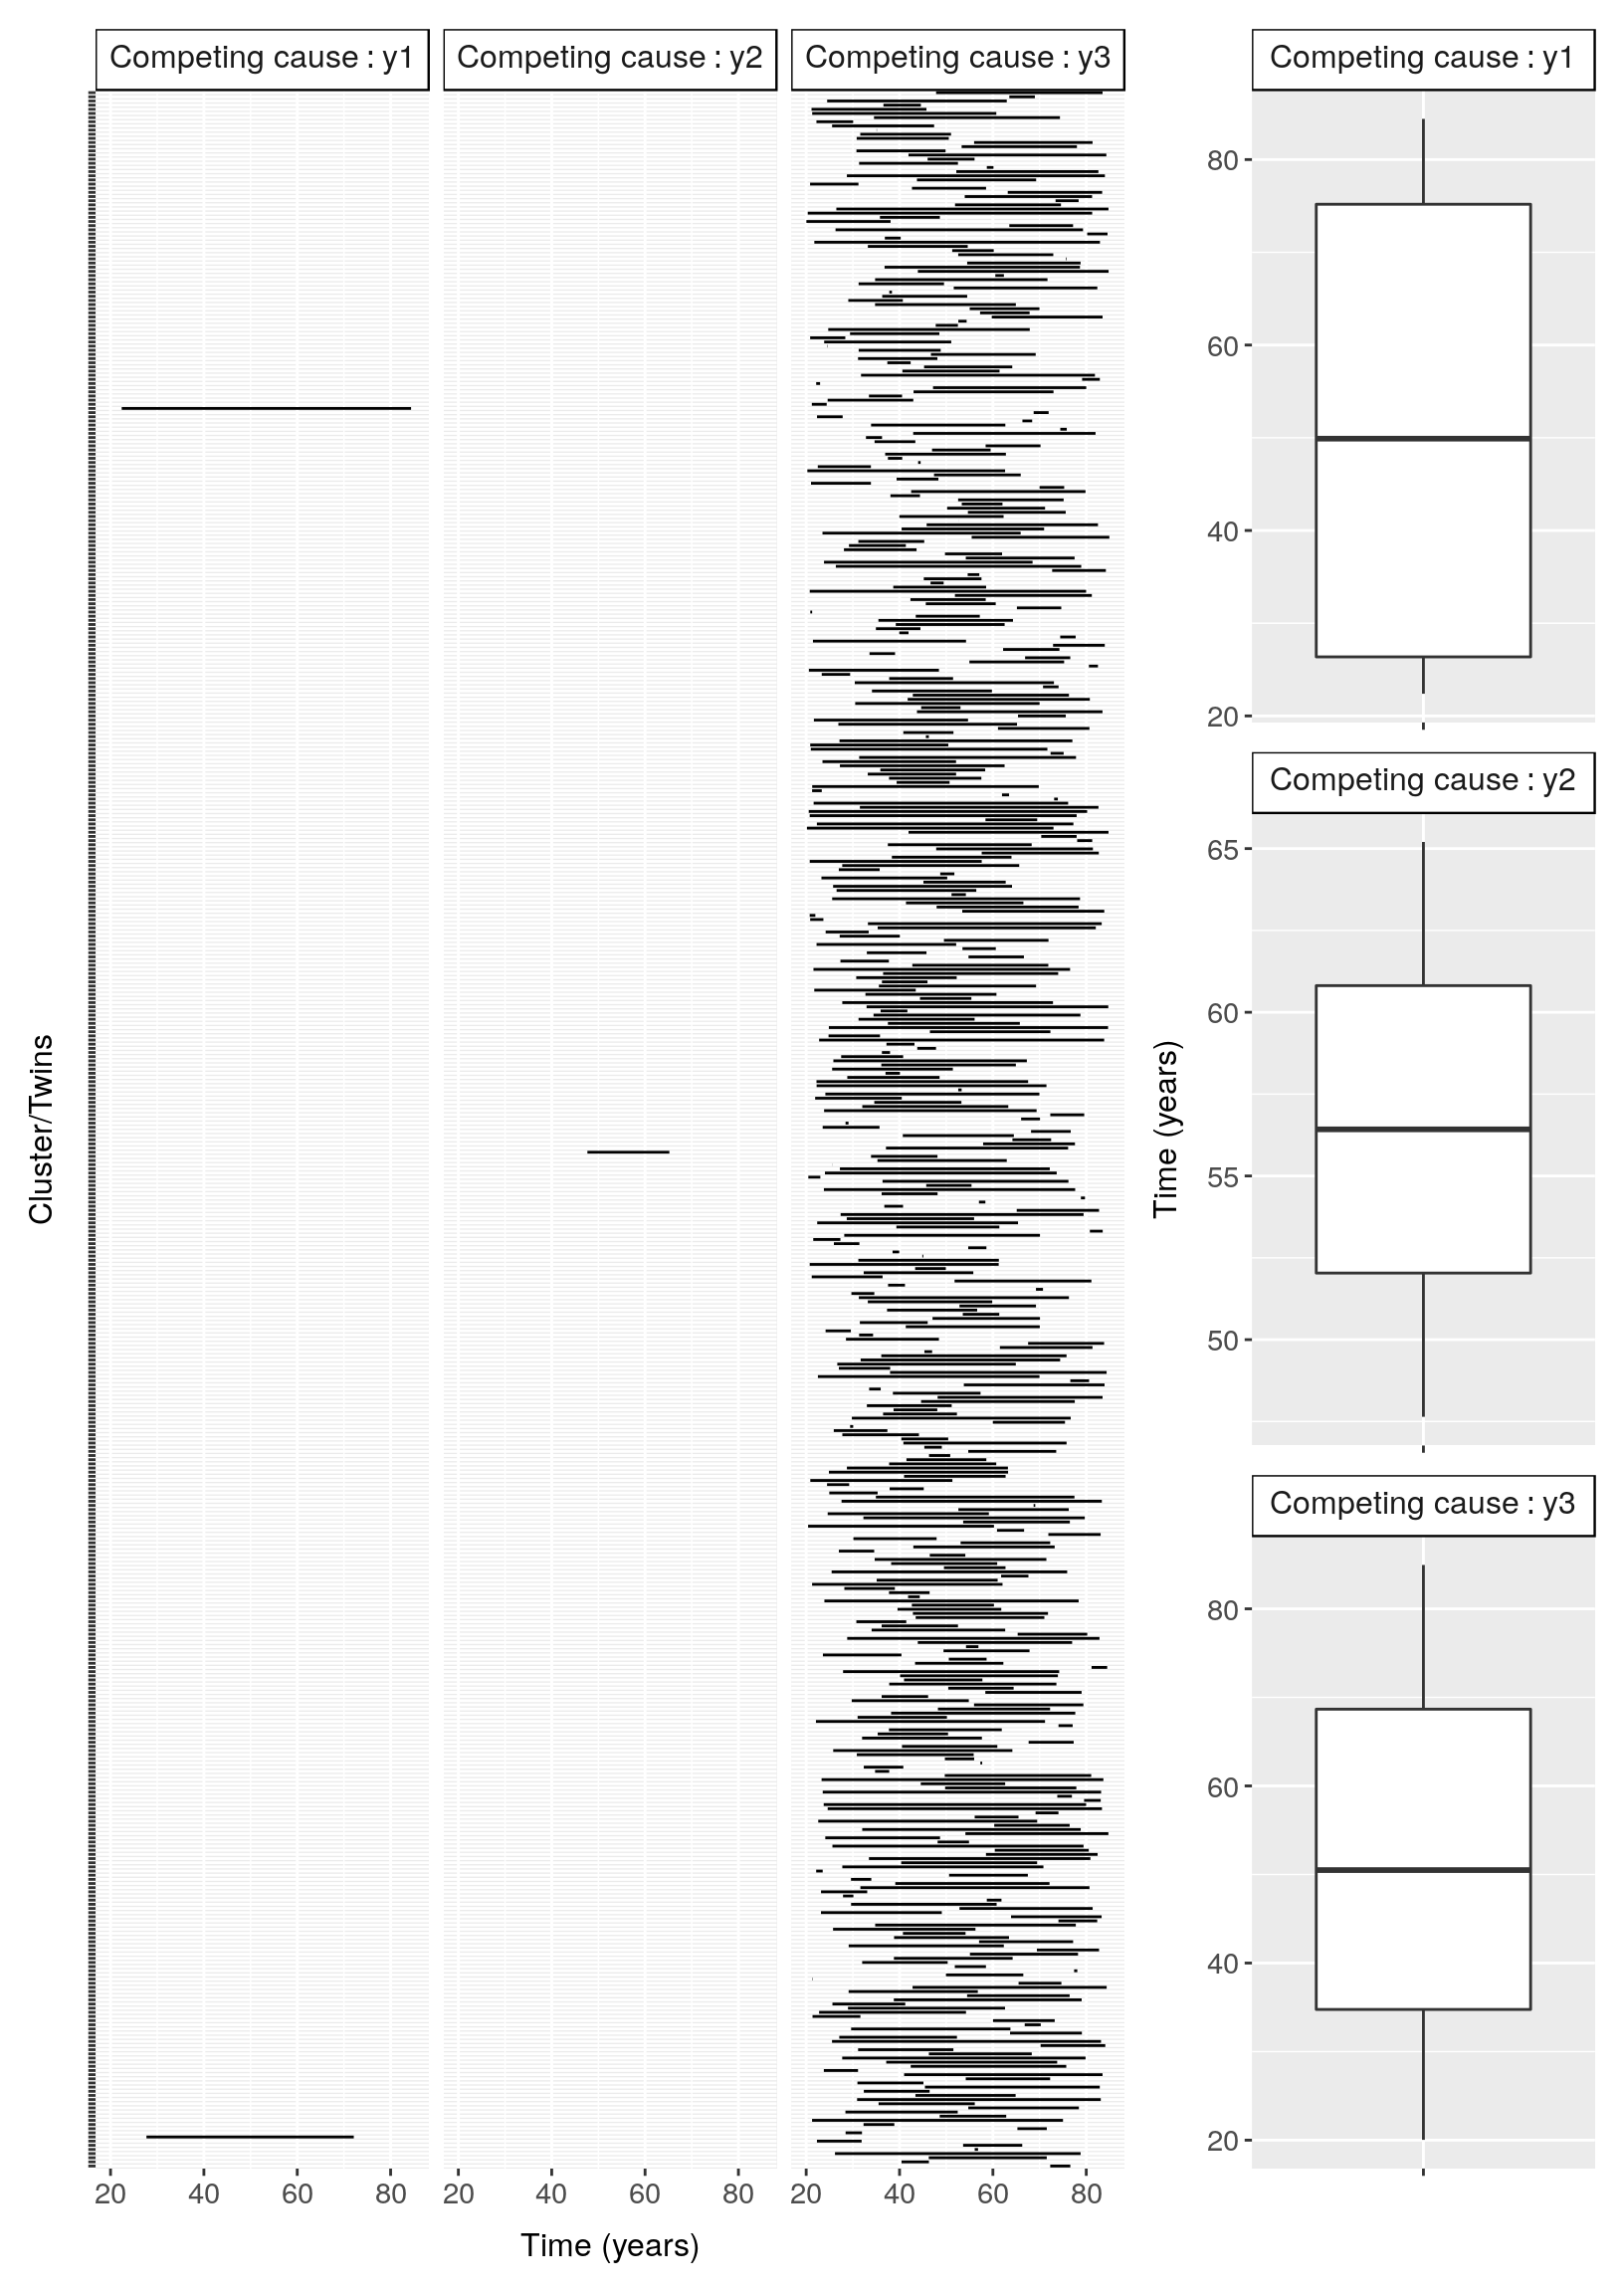
\includegraphics[width=\textwidth]{datasimu-1.png}
  \\
  \vspace{0.45cm}
  \begin{footnotesize}
    SOURCE: The author (2020).
  \end{footnotesize}
  \label{fig:datasimu}
\end{figure}

\begin{figure}[H]
  \vspace{0.35cm}
  \setlength{\abovecaptionskip}{.00001pt}
  \caption{CÓDIGOS EM LINGUAGEM R PARA GERAÇÃO DE VARIÁVEIS ALEATÓRIAS
    BETA CORRELACIONADAS}
  \vspace{-0.25cm}
  \begin{program}[H]
    \begin{tikzpicture}
      \node [mybox] (box){
        \begin{minipage}{0.955\textwidth}
\begin{verbatim}
R = 1000  # tamanho da amostra
mu = 0.5  # parâmetro de média
phi = 9  # parâmetro de dispersão
cor_matrix <- matrix(c(1.0,0.75,0.75,1.0),2,2) # matriz de correlação
require(MASS)  # carrega o pacote com a função mvrnorm()
Z <- mvrnorm(n = R, mu = c(0,0), Sigma = cor_matrix)  # passo 1
Y <- qbeta(pnorm(Z), shape1 = mu*phi, shape2 = (1 - mu)*phi) # passo 2
\end{verbatim}
        \end{minipage}
      };
    \end{tikzpicture}
  \end{program}
  % \vspace{-.75cm}
  \begin{footnotesize}
    \begin{center}
      SOURCE: The author (2020).
    \end{center}
  \end{footnotesize}
  \label{fig:steps1e2}
\end{figure}

\section{REAL-BASED DATASET}
\label{cap:data}

% END ==================================================================